\documentclass[12pt, a4paper]{book}
\usepackage[T1]{fontenc}
\usepackage[utf8]{inputenc}
\usepackage[charter, cal=cmcal]{mathdesign}
\usepackage[scaled=0.92]{helvet}
\usepackage{geometry}
\geometry{a4paper, top=30mm, bottom=30mm, inner=32mm, outer=25mm}
\usepackage{amsmath, amssymb}
\usepackage[version=4]{mhchem}
\usepackage[dvipsnames,svgnames,table]{xcolor}
\usepackage{tikz}
\usetikzlibrary{arrows.meta, positioning, calc, backgrounds, decorations.pathmorphing}
\usepackage{pgfplots}
\pgfplotsset{compat=1.18}
\usepackage{tcolorbox}
\tcbuselibrary{skins, breakable}
\usepackage{titlesec}
\usepackage{fancyhdr}
\usepackage{enumitem}
\usepackage{booktabs}
\usepackage{array}
\usepackage{parskip}
\usepackage{siunitx}
\usepackage[colorlinks=true, linkcolor=BrickRed, urlcolor=NavyBlue]{hyperref}

\definecolor{JourneyColor}{HTML}{1A5276}
\definecolor{ModuleColor}{HTML}{2E86C1}
\definecolor{PuzzleColor}{HTML}{145A32}
\definecolor{DiscoveryColor}{HTML}{B7950B}
\definecolor{WarningColor}{HTML}{C0392B}
\definecolor{ProblemColor}{HTML}{4A235A}
\definecolor{ReflectColor}{HTML}{117A65}
\definecolor{HistoryColor}{HTML}{6E2F1A}
\definecolor{BondingColor}{HTML}{1A5276}
\definecolor{AntibondColor}{HTML}{922B21}
\definecolor{SigmaColor}{HTML}{1E8449}
\definecolor{PiColor}{HTML}{7D3C98}

\newtcolorbox{puzzlebox}[1][]{enhanced,breakable,
  colback=PuzzleColor!6,colframe=PuzzleColor,fonttitle=\bfseries\sffamily,
  title={The Puzzle},attach boxed title to top left={yshift=-2mm,xshift=6mm},
  boxed title style={colback=PuzzleColor},borderline west={3pt}{0pt}{PuzzleColor},#1}
\newtcolorbox{discoverybox}[1][]{enhanced,breakable,
  colback=DiscoveryColor!8,colframe=DiscoveryColor,fonttitle=\bfseries\sffamily,
  title={Discovery},attach boxed title to top left={yshift=-2mm,xshift=6mm},
  boxed title style={colback=DiscoveryColor},borderline west={3pt}{0pt}{DiscoveryColor},#1}
\newtcolorbox{problembox}[1][]{enhanced,breakable,
  colback=ProblemColor!5,colframe=ProblemColor,fonttitle=\bfseries\sffamily,
  title={Problems},attach boxed title to top left={yshift=-2mm,xshift=6mm},
  boxed title style={colback=ProblemColor},borderline west={3pt}{0pt}{ProblemColor},#1}
\newtcolorbox{deepbox}[1][]{enhanced,breakable,
  colback=JourneyColor!5,colframe=JourneyColor,fonttitle=\bfseries\sffamily,
  title={Deep Problems},attach boxed title to top left={yshift=-2mm,xshift=6mm},
  boxed title style={colback=JourneyColor},borderline west={4pt}{0pt}{JourneyColor},#1}
\newtcolorbox{reflectionbox}[1][]{enhanced,breakable,
  colback=ReflectColor!6,colframe=ReflectColor,fonttitle=\bfseries\sffamily,
  title={Reflection},attach boxed title to top left={yshift=-2mm,xshift=6mm},
  boxed title style={colback=ReflectColor},borderline west={3pt}{0pt}{ReflectColor},#1}
\newtcolorbox{namedconcept}[2][]{enhanced,
  colback=ModuleColor!6,colframe=ModuleColor,fonttitle=\bfseries\sffamily\large,
  title={#2},attach boxed title to top left={yshift=-2mm,xshift=6mm},
  boxed title style={colback=ModuleColor},#1}
\newtcolorbox{modelbreaks}[1][]{enhanced,breakable,
  colback=WarningColor!6,colframe=WarningColor,fonttitle=\bfseries\sffamily,
  title={Where This Model Breaks},attach boxed title to top left={yshift=-2mm,xshift=6mm},
  boxed title style={colback=WarningColor},borderline west={4pt}{0pt}{WarningColor},#1}

\titleformat{\chapter}[display]
  {\normalfont\sffamily\huge\bfseries\color{JourneyColor}}
  {\textcolor{JourneyColor!60}{\chaptertitlename\ \thechapter}}{10pt}{\Huge}
  [\vspace{2pt}\textcolor{JourneyColor}{\titlerule[1.5pt]}]
\titleformat{\section}{\normalfont\sffamily\Large\bfseries\color{ModuleColor}}
  {\thesection}{1em}{}[\textcolor{ModuleColor!40}{\titlerule[0.6pt]}]
\titleformat{\subsection}{\normalfont\sffamily\large\bfseries\color{JourneyColor!80}}
  {\thesubsection}{1em}{}
\pagestyle{fancy}\fancyhf{}
\fancyhead[LE]{\small\sffamily\textcolor{JourneyColor}{\leftmark}}
\fancyhead[RO]{\small\sffamily\textcolor{ModuleColor}{\rightmark}}
\fancyfoot[C]{\small\thepage}
\renewcommand{\headrulewidth}{0.4pt}
\newcommand{\newterm}[1]{\textit{\textcolor{DiscoveryColor}{#1}}}

% ══════════════════════════════════════════════════════════════════════════════
\begin{document}
\setcounter{chapter}{3}
\chapter[Journey 4 --- The Bond]{Journey Four\\[8pt]
  \textcolor{ModuleColor}{\large The Bond: Why Atoms Stick Together}}
\setcounter{section}{2}

\section{Module 4.3 --- Covalent Bonding: Orbitals Overlapping}

\subsection*{Motivation}

The ionic model works beautifully for NaCl.
But it fails completely for \ce{H2}, \ce{O2}, \ce{N2},
and the vast majority of compounds in organic chemistry,
biochemistry, and materials science.

In these molecules, atoms share electrons rather than
transfer them.
The quantum mechanical description of electron sharing
is \newterm{molecular orbital (MO) theory}:
atomic orbitals combine to form molecular orbitals
that span the entire molecule.

This module builds MO theory from its foundation ---
constructive and destructive interference of wave functions ---
up through sigma and pi bonds, bond order, and the
explanation of the unexpected paramagnetism of \ce{O2}.

\subsection{From Atomic to Molecular Orbitals}

Atomic orbitals are wave functions.
When two atoms approach, their wave functions overlap.
Just as two waves can add constructively or destructively,
two atomic orbitals combine in two ways:

\begin{center}
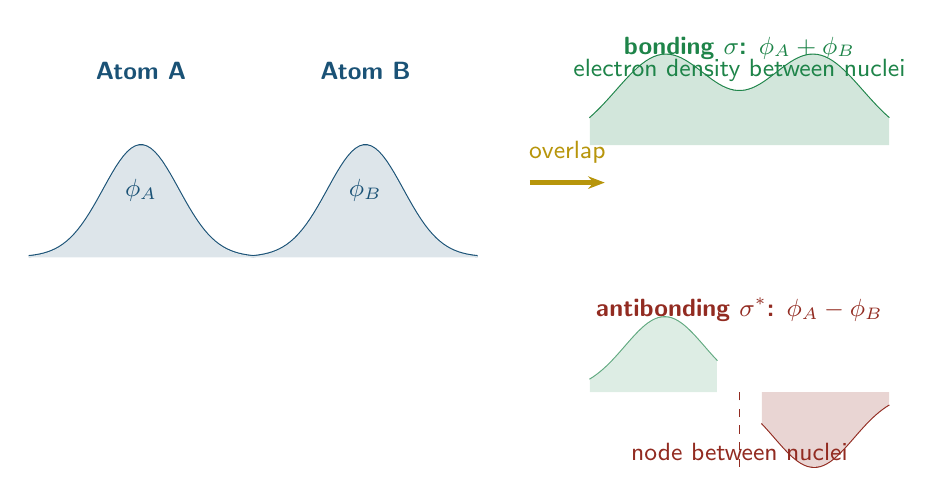
\begin{tikzpicture}[every node/.style={font=\sffamily\small}, scale=0.95]

  % Atom A orbital (1s-like)
  \begin{scope}[xshift=0cm]
    \node[font=\sffamily\small\bfseries, color=JourneyColor]
      at (0, 2.5) {Atom A};
    \draw[thick, BondingColor]
      plot[domain=-1.5:1.5, samples=60]
        (\x, {1.5*exp(-2*\x*\x)});
    \fill[BondingColor!15]
      plot[domain=-1.5:1.5, samples=60]
        (\x, {1.5*exp(-2*\x*\x)})
      -- (1.5,0) -- (-1.5,0) -- cycle;
    \node[font=\sffamily\small, text=BondingColor] at (0,0.9) {$\phi_A$};
  \end{scope}

  % Atom B orbital
  \begin{scope}[xshift=3.0cm]
    \node[font=\sffamily\small\bfseries, color=JourneyColor]
      at (0, 2.5) {Atom B};
    \draw[thick, BondingColor]
      plot[domain=-1.5:1.5, samples=60]
        (\x, {1.5*exp(-2*\x*\x)});
    \fill[BondingColor!15]
      plot[domain=-1.5:1.5, samples=60]
        (\x, {1.5*exp(-2*\x*\x)})
      -- (1.5,0) -- (-1.5,0) -- cycle;
    \node[font=\sffamily\small, text=BondingColor] at (0,0.9) {$\phi_B$};
  \end{scope}

  % Addition arrow
  \draw[-{Stealth[length=6pt]}, ultra thick, DiscoveryColor]
    (5.2, 1.0) -- (6.2, 1.0);
  \node[font=\sffamily\small, text=DiscoveryColor] at (5.7, 1.4) {overlap};

  % Bonding MO (constructive)
  \begin{scope}[xshift=6.5cm, yshift=1.5cm]
    \node[font=\sffamily\small\bfseries, color=SigmaColor]
      at (1.5, 1.3) {bonding $\sigma$: $\phi_A + \phi_B$};
    \draw[thick, SigmaColor]
      plot[domain=-0.5:3.5, samples=80]
        (\x, {1.2*exp(-1.2*(\x-0.5)*(\x-0.5))
              + 1.2*exp(-1.2*(\x-2.5)*(\x-2.5))});
    \fill[SigmaColor!20]
      plot[domain=-0.5:3.5, samples=80]
        (\x, {1.2*exp(-1.2*(\x-0.5)*(\x-0.5))
              + 1.2*exp(-1.2*(\x-2.5)*(\x-2.5))})
      -- (3.5,0) -- (-0.5,0) -- cycle;
    \node[font=\sffamily\small, text=SigmaColor] at (1.5,1.0)
      {electron density between nuclei};
  \end{scope}

  % Antibonding MO (destructive)
  \begin{scope}[xshift=6.5cm, yshift=-1.8cm]
    \node[font=\sffamily\small\bfseries, color=AntibondColor]
      at (1.5, 1.1) {antibonding $\sigma^*$: $\phi_A - \phi_B$};
    \draw[thick, SigmaColor!70]
      plot[domain=-0.5:1.2, samples=40]
        (\x, {1.0*exp(-1.8*(\x-0.5)*(\x-0.5))});
    \fill[SigmaColor!15]
      plot[domain=-0.5:1.2, samples=40]
        (\x, {1.0*exp(-1.8*(\x-0.5)*(\x-0.5))})
      -- (1.2,0) -- (-0.5,0) -- cycle;
    \draw[thick, AntibondColor]
      plot[domain=1.8:3.5, samples=40]
        (\x, {-1.0*exp(-1.8*(\x-2.5)*(\x-2.5))});
    \fill[AntibondColor!20]
      plot[domain=1.8:3.5, samples=40]
        (\x, {-1.0*exp(-1.8*(\x-2.5)*(\x-2.5))})
      -- (3.5,0) -- (1.8,0) -- cycle;
    \node[font=\sffamily\small, text=AntibondColor] at (1.5,-0.8)
      {node between nuclei};
    \draw[dashed, thin, AntibondColor] (1.5,-1.0) -- (1.5,0.0);
  \end{scope}

\end{tikzpicture}
\end{center}

\begin{namedconcept}{Linear Combination of Atomic Orbitals (LCAO)}
When $N$ atomic orbitals combine, they produce $N$ molecular orbitals:
\begin{align*}
  \psi_\text{bonding}     &= \phi_A + \phi_B
    \quad \text{(constructive, lower energy)} \\
  \psi_\text{antibonding} &= \phi_A - \phi_B
    \quad \text{(destructive, higher energy)}
\end{align*}

The bonding MO has electron density \emph{between} the nuclei
--- electrons there are attracted to both nuclei simultaneously.

The antibonding MO has a \emph{node} between the nuclei
--- placing electrons there destabilises the molecule.

The energy splitting is proportional to the overlap integral
$S = \int \phi_A \phi_B\, dV$: greater overlap means larger splitting.
\end{namedconcept}

\subsection{MO Diagrams for Homonuclear Diatomics}

For Period-2 homonuclear diatomics (\ce{Li2} through \ce{Ne2}),
we combine the $2s$ and $2p$ atomic orbitals.
Each atom contributes four valence orbitals ($2s$, $2p_x$, $2p_y$, $2p_z$),
giving 8 molecular orbitals total.

\begin{center}
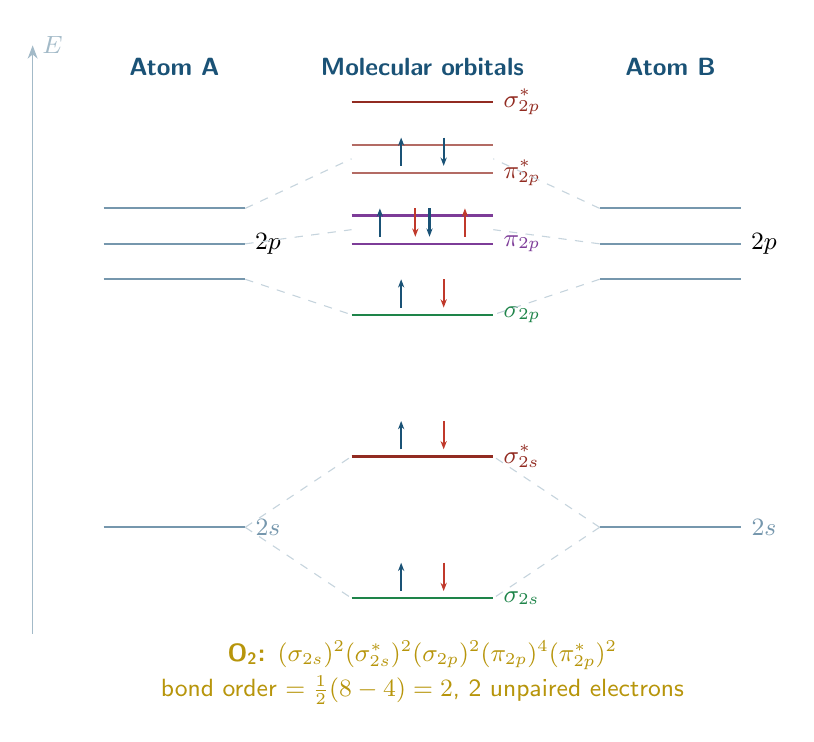
\begin{tikzpicture}[every node/.style={font=\sffamily\small}, scale=0.9]

  % Atom A levels (left)
  \node[font=\sffamily\small\bfseries, color=JourneyColor]
    at (-3.5, 7.5) {Atom A};
  % 2s
  \draw[thick, BondingColor!60] (-4.5,1.0) -- (-2.5,1.0)
    node[right, font=\sffamily\small] {$2s$};
  % 2p (degenerate trio)
  \foreach \y in {4.5,5.0,5.5} {
    \draw[thick, BondingColor!60] (-4.5,\y) -- (-2.5,\y);
  }
  \node[right, font=\sffamily\small] at (-2.5,5.0) {$2p$};

  % Atom B levels (right)
  \node[font=\sffamily\small\bfseries, color=JourneyColor]
    at (3.5, 7.5) {Atom B};
  \draw[thick, BondingColor!60] (2.5,1.0) -- (4.5,1.0)
    node[right, font=\sffamily\small] {$2s$};
  \foreach \y in {4.5,5.0,5.5} {
    \draw[thick, BondingColor!60] (2.5,\y) -- (4.5,\y);
  }
  \node[right, font=\sffamily\small] at (4.5,5.0) {$2p$};

  % MO levels (centre) -- ordering for O2, F2 (no 2s-2p mixing)
  \node[font=\sffamily\small\bfseries, color=JourneyColor]
    at (0, 7.5) {Molecular orbitals};
  % sigma_2s bonding
  \draw[thick, SigmaColor] (-1.0,0.0) -- (1.0,0.0)
    node[right, font=\sffamily\small, text=SigmaColor] {$\sigma_{2s}$};
  % sigma*_2s antibonding
  \draw[thick, AntibondColor] (-1.0,2.0) -- (1.0,2.0)
    node[right, font=\sffamily\small, text=AntibondColor] {$\sigma^*_{2s}$};
  % sigma_2p bonding
  \draw[thick, SigmaColor] (-1.0,4.0) -- (1.0,4.0)
    node[right, font=\sffamily\small, text=SigmaColor] {$\sigma_{2p}$};
  % pi_2p bonding (degenerate pair)
  \draw[thick, PiColor] (-1.0,5.0) -- (1.0,5.0)
    node[right, font=\sffamily\small, text=PiColor] {$\pi_{2p}$};
  \draw[thick, PiColor] (-1.0,5.4) -- (1.0,5.4);
  % pi*_2p antibonding (degenerate pair)
  \draw[thick, AntibondColor!70] (-1.0,6.0) -- (1.0,6.0)
    node[right, font=\sffamily\small, text=AntibondColor] {$\pi^*_{2p}$};
  \draw[thick, AntibondColor!70] (-1.0,6.4) -- (1.0,6.4);
  % sigma*_2p antibonding
  \draw[thick, AntibondColor] (-1.0,7.0) -- (1.0,7.0)
    node[right, font=\sffamily\small, text=AntibondColor] {$\sigma^*_{2p}$};

  % Connecting dashed lines (atom A to MO)
  \draw[dashed, thin, JourneyColor!25] (-2.5,1.0)  -- (-1.0,0.0);
  \draw[dashed, thin, JourneyColor!25] (-2.5,1.0)  -- (-1.0,2.0);
  \draw[dashed, thin, JourneyColor!25] (-2.5,4.5)  -- (-1.0,4.0);
  \draw[dashed, thin, JourneyColor!25] (-2.5,5.0)  -- (-1.0,5.2);
  \draw[dashed, thin, JourneyColor!25] (-2.5,5.5)  -- (-1.0,6.2);
  % Connecting dashed lines (atom B to MO)
  \draw[dashed, thin, JourneyColor!25] (2.5,1.0)   -- (1.0,0.0);
  \draw[dashed, thin, JourneyColor!25] (2.5,1.0)   -- (1.0,2.0);
  \draw[dashed, thin, JourneyColor!25] (2.5,4.5)   -- (1.0,4.0);
  \draw[dashed, thin, JourneyColor!25] (2.5,5.0)   -- (1.0,5.2);
  \draw[dashed, thin, JourneyColor!25] (2.5,5.5)   -- (1.0,6.2);

  % Energy axis
  \draw[-{Stealth}, thin, JourneyColor!40]
    (-5.5,-0.5) -- (-5.5,7.8)
    node[right, font=\sffamily\small] {$E$};

  % O2 electrons (fill up to sigma*_2p half-filled)
  % sigma_2s: 2 up/down
  \draw[-{Stealth[length=3pt]},thick,BondingColor] (-0.3,0.1)--(-0.3,0.5);
  \draw[-{Stealth[length=3pt]},thick,WarningColor] (0.3,0.5)--(0.3,0.1);
  % sigma*_2s: 2
  \draw[-{Stealth[length=3pt]},thick,BondingColor] (-0.3,2.1)--(-0.3,2.5);
  \draw[-{Stealth[length=3pt]},thick,WarningColor] (0.3,2.5)--(0.3,2.1);
  % sigma_2p: 2
  \draw[-{Stealth[length=3pt]},thick,BondingColor] (-0.3,4.1)--(-0.3,4.5);
  \draw[-{Stealth[length=3pt]},thick,WarningColor] (0.3,4.5)--(0.3,4.1);
  % pi_2p: 4 (2 per orbital)
  \draw[-{Stealth[length=3pt]},thick,BondingColor] (-0.6,5.1)--(-0.6,5.5);
  \draw[-{Stealth[length=3pt]},thick,WarningColor] (-0.1,5.5)--(-0.1,5.1);
  \draw[-{Stealth[length=3pt]},thick,BondingColor] (0.1,5.5)--(0.1,5.1);
  \draw[-{Stealth[length=3pt]},thick,WarningColor] (0.6,5.1)--(0.6,5.5);
  % pi*_2p: 2, one in each (Hund's rule) -- THIS is why O2 is paramagnetic
  \draw[-{Stealth[length=3pt]},thick,BondingColor] (-0.3,6.1)--(-0.3,6.5);
  \draw[-{Stealth[length=3pt]},thick,BondingColor] (0.3,6.5)--(0.3,6.1);

  % O2 label
  \node[font=\sffamily\small\bfseries, text=DiscoveryColor]
    at (0,-0.8) {\ce{O2}: $(\sigma_{2s})^2(\sigma^*_{2s})^2(\sigma_{2p})^2
    (\pi_{2p})^4(\pi^*_{2p})^2$};
  \node[font=\sffamily\small, text=DiscoveryColor]
    at (0,-1.3) {bond order $= \frac{1}{2}(8-4) = 2$, 2 unpaired electrons};

\end{tikzpicture}
\end{center}

\vspace{0.4em}

The MO diagram immediately explains the famous puzzle of \ce{O2}:
Lewis structures predict all electrons paired (diamagnetic),
but \ce{O2} is \textbf{paramagnetic} with two unpaired electrons.
The MO diagram shows why: the two electrons entering
$\pi^*_{2p}$ go into separate (degenerate) orbitals
by Hund's rule, giving two unpaired spins.
This was a spectacular early success of MO theory.

\subsection{Bond Order, Length, and Energy from MO Theory}

\begin{namedconcept}{Bond Order in MO Theory}
\[
  \text{Bond order} = \frac{1}{2}(\text{bonding electrons}
                                  - \text{antibonding electrons})
\]
A bond order of 1 corresponds to a single bond;
2 to a double bond; 3 to a triple bond.
Bond order 0 means the molecule does not exist
(or only as a very weakly bound species).
\end{namedconcept}

\begin{center}
\small
\begin{tabular}{lllccc}
\toprule
Molecule & Config (valence) & Bond order & Length (pm) & Energy (kJ/mol) & Magnetic \\
\midrule
\ce{H2+}  & $(\sigma_{1s})^1$                   & 0.5 & 106 & 255 & paramagnetic \\
\ce{H2}   & $(\sigma_{1s})^2$                   & 1   & 74  & 432 & diamagnetic \\
\ce{He2+} & $(\sigma_{1s})^2(\sigma^*_{1s})^1$  & 0.5 & 108 & 251 & paramagnetic \\
\ce{He2}  & $(\sigma_{1s})^2(\sigma^*_{1s})^2$  & 0   & ---  & --- & does not exist \\
\ce{Li2}  & $(\sigma_{2s})^2$                   & 1   & 267 & 105 & diamagnetic \\
\ce{N2}   & $\ldots(\sigma_{2p})^2(\pi_{2p})^4$ & 3   & 110 & 945 & diamagnetic \\
\ce{O2}   & $\ldots(\pi_{2p})^4(\pi^*_{2p})^2$ & 2   & 121 & 498 & paramagnetic \\
\ce{F2}   & $\ldots(\pi^*_{2p})^4$              & 1   & 141 & 159 & diamagnetic \\
\ce{Ne2}  & $\ldots(\sigma^*_{2p})^2$           & 0   & ---  & --- & does not exist \\
\bottomrule
\end{tabular}
\end{center}

\vspace{0.5em}

The trend is clear and quantitative:
higher bond order correlates with shorter, stronger bonds.
\ce{N2} (bond order 3) is the strongest diatomic bond known.
\ce{F2} (bond order 1, but with many filled antibonding orbitals)
is surprisingly weak: all those antibonding electrons
nearly cancel the bonding ones.

\subsection{Sigma and Pi Bonds: Symmetry of Overlap}

\begin{center}
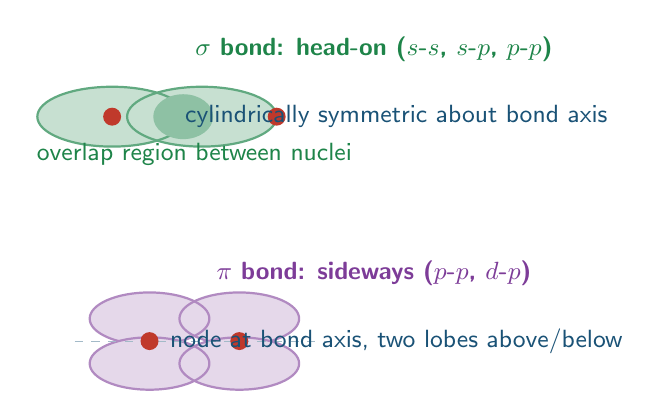
\begin{tikzpicture}[every node/.style={font=\sffamily\small}, scale=0.95]

  % Sigma bond: head-on overlap of p orbitals along bond axis
  \begin{scope}[yshift=2.5cm]
    \node[font=\sffamily\small\bfseries, color=SigmaColor]
      at (3.5,1.4) {$\sigma$ bond: head-on ($s$-$s$, $s$-$p$, $p$-$p$)};
    % Left lobe
    \fill[SigmaColor!25] (0.0,0.5) ellipse (1.0cm and 0.4cm);
    \fill[SigmaColor!25] (1.2,0.5) ellipse (1.0cm and 0.4cm);
    \draw[thick,SigmaColor!70] (0.0,0.5) ellipse (1.0cm and 0.4cm);
    \draw[thick,SigmaColor!70] (1.2,0.5) ellipse (1.0cm and 0.4cm);
    % Nuclei
    \fill[WarningColor] (0.0,0.5) circle (0.12cm);
    \fill[WarningColor] (2.2,0.5) circle (0.12cm);
    % Overlap annotation
    \fill[SigmaColor!50] (0.95,0.5) ellipse (0.4cm and 0.3cm);
    \node[font=\sffamily\small, text=SigmaColor] at (1.1,0.0)
      {overlap region between nuclei};
    \node[font=\sffamily\small, text=JourneyColor] at (3.8,0.5)
      {cylindrically symmetric about bond axis};
  \end{scope}

  % Pi bond: sideways overlap of p orbitals
  \begin{scope}[yshift=-0.5cm]
    \node[font=\sffamily\small\bfseries, color=PiColor]
      at (3.5,1.4) {$\pi$ bond: sideways ($p$-$p$, $d$-$p$)};
    % Above axis
    \fill[PiColor!20] (0.5,0.8) ellipse (0.8cm and 0.35cm);
    \fill[PiColor!20] (1.7,0.8) ellipse (0.8cm and 0.35cm);
    \draw[thick,PiColor!60] (0.5,0.8) ellipse (0.8cm and 0.35cm);
    \draw[thick,PiColor!60] (1.7,0.8) ellipse (0.8cm and 0.35cm);
    % Below axis
    \fill[PiColor!20] (0.5,0.2) ellipse (0.8cm and 0.35cm);
    \fill[PiColor!20] (1.7,0.2) ellipse (0.8cm and 0.35cm);
    \draw[thick,PiColor!60] (0.5,0.2) ellipse (0.8cm and 0.35cm);
    \draw[thick,PiColor!60] (1.7,0.2) ellipse (0.8cm and 0.35cm);
    % Bond axis (nodal plane)
    \draw[dashed, thin, JourneyColor!40] (-0.5,0.5) -- (3.0,0.5);
    % Nuclei
    \fill[WarningColor] (0.5,0.5) circle (0.12cm);
    \fill[WarningColor] (1.7,0.5) circle (0.12cm);
    \node[font=\sffamily\small, text=JourneyColor] at (3.8,0.5)
      {node at bond axis, two lobes above/below};
  \end{scope}

\end{tikzpicture}
\end{center}

Key differences between $\sigma$ and $\pi$ bonds:
\begin{itemize}[nosep, leftmargin=2em]
  \item $\sigma$ bonds have electron density \emph{along} the
        internuclear axis; rotation about the bond is free.
  \item $\pi$ bonds have electron density \emph{above and below}
        the axis; rotation about the bond is \textbf{restricted}
        (breaking the $\pi$ bond requires $\sim 260$ kJ/mol).
        This is why \ce{C=C} double bonds can exist as
        \textit{cis}/\textit{trans} isomers.
  \item $\sigma$ bonds are stronger than $\pi$ bonds (better overlap).
  \item A double bond = one $\sigma$ + one $\pi$.
        A triple bond = one $\sigma$ + two $\pi$.
\end{itemize}

\subsection{Hybridisation: Reconciling Geometry with MO Theory}

Methane (\ce{CH4}) has four identical C--H bonds at
$109.5^\circ$ angles.
But carbon's ground-state configuration is $2s^2\,2p^2$ ---
only two unpaired $p$ electrons available for bonding.

The resolution: before bonding, the $2s$ and $2p$ orbitals
on carbon \newterm{hybridise} --- mix to form four new orbitals
pointing toward the corners of a tetrahedron.

\begin{center}
\small
\begin{tabular}{lllll}
\toprule
Hybridisation & Geometry & Bond angles & Example & Unhybridised \\
\midrule
$sp^3$ & tetrahedral    & $109.5^\circ$ & \ce{CH4}, \ce{NH3} & none \\
$sp^2$ & trigonal planar& $120^\circ$   & \ce{CH2=CH2}, \ce{BF3} & 1 $p$ orbital (forms $\pi$) \\
$sp$   & linear         & $180^\circ$   & HC$\equiv$CH, \ce{CO2} & 2 $p$ orbitals (2 $\pi$ bonds) \\
$d^2sp^3$ & octahedral  & $90^\circ$    & \ce{SF6} & none \\
\bottomrule
\end{tabular}
\end{center}

\vspace{0.3em}

Hybridisation is a mathematical transformation:
the hybridised orbitals are linear combinations of the
atomic ones.
For $sp^3$:
\[
  h_1 = \tfrac{1}{2}(s + p_x + p_y + p_z), \quad
  h_2 = \tfrac{1}{2}(s + p_x - p_y - p_z), \quad
  \ldots
\]
These four combinations point in tetrahedral directions
and overlap more effectively with H $1s$ orbitals
than the pure $p$ orbitals would.

\begin{problembox}
\begin{enumerate}[label=\textbf{\arabic*.}]
  \item \textbf{MO diagrams and bond properties.}

    Complete the MO electron configurations and calculate
    bond orders for:
    \begin{enumerate}[label=(\alph*)]
      \item \ce{N2+} (remove one electron from \ce{N2})
      \item \ce{O2+} (remove one electron from \ce{O2})
      \item \ce{O2-} (add one electron to \ce{O2})
      \item \ce{O2^{2-}} (add two electrons to \ce{O2})
    \end{enumerate}
    For each: state bond order, predict whether bond is
    longer or shorter than the neutral molecule, and state
    whether paramagnetic or diamagnetic.

  \item \textbf{The weakness of F$_2$.}

    \ce{F2} (bond energy 159 kJ/mol) is weaker than
    \ce{Cl2} (242 kJ/mol) despite F being more electronegative.
    This seems paradoxical: shouldn't a more electronegative
    atom form stronger bonds?

    \begin{enumerate}[label=(\alph*)]
      \item Using the MO diagram, count the bonding and
            antibonding electrons in \ce{F2}.
            How many antibonding electrons destabilise the bond?
      \item The lone pairs on F occupy $2p$ orbitals.
            When the two F atoms approach, these $2p$ lone
            pairs also overlap --- in an antibonding fashion.
            Explain how lone pair--lone pair repulsion
            weakens the F--F bond.
      \item Why does this effect not weaken Cl--Cl as much?
            (Hint: the lone pairs are in $3p$ orbitals,
            farther from the nucleus, less compact.)
    \end{enumerate}

  \item \textbf{Hybridisation and geometry.}

    Predict the hybridisation of the central atom and
    the molecular geometry of:
    \begin{enumerate}[label=(\alph*)]
      \item \ce{BCl3} (boron has no lone pairs)
      \item \ce{PCl5} (phosphorus uses $d$ orbitals)
      \item \ce{XeF2} (from Module 3.3)
      \item \ce{CO2}
      \item \ce{SO3}
    \end{enumerate}
    For each: draw the Lewis structure, identify lone pairs
    on the central atom, state hybridisation, and name the geometry.
\end{enumerate}
\end{problembox}

\subsection*{Where MO Theory Breaks Down}

\begin{modelbreaks}
\begin{itemize}[nosep, leftmargin=2em]
  \item \textbf{Computational cost.} The full MO treatment of a
        large molecule requires solving the many-electron
        Schr\"{o}dinger equation, which scales as $O(N^3)$
        or worse with the number of electrons $N$.
        For proteins (thousands of atoms), exact MO theory
        is computationally impossible; approximations
        (density functional theory, semiempirical methods)
        are used instead.

  \item \textbf{Localised bonds.} MO theory produces delocalised
        orbitals spanning the whole molecule.
        In practice, many bonds (C--H in methane, for example)
        behave as though localised between two atoms.
        Valence bond (VB) theory handles this more naturally,
        but VB is less systematic.

  \item \textbf{Strong correlation.} In molecules with
        near-degenerate configurations (e.g.\ transition metal
        complexes, biradicals), single-determinant MO theory
        fails qualitatively.
        Multi-reference methods (CASSCF, MRCI) are needed
        but are expensive.

  \item \textbf{Crossing of MO ordering.} For \ce{Li2} through
        \ce{N2}, the $\pi_{2p}$ levels are actually
        \emph{lower} in energy than $\sigma_{2p}$ due to
        $2s$-$2p$ mixing (these are close in energy for
        light atoms).
        For \ce{O2} and \ce{F2}, $\sigma_{2p} < \pi_{2p}$.
        The simple diagram above applies only to \ce{O2}/\ce{F2}.
\end{itemize}
\end{modelbreaks}

\subsection*{Deep Problems}

\begin{deepbox}
\begin{enumerate}[label=\textbf{D\arabic*.}]

  \item \textbf{\ce{O2} paramagnetism: the historical significance.}

    Before MO theory, Linus Pauling and others used Lewis
    structures and valence bond theory to describe bonding.
    The Lewis structure of \ce{O2} (\ce{O=O}) predicts all
    electrons paired and thus diamagnetic.
    But liquid \ce{O2} poured between the poles of a strong
    magnet hangs between them --- it is paramagnetic.

    \begin{enumerate}[label=(\alph*)]
      \item Describe the experimental test: if \ce{O2} is
            poured between two strong magnet poles,
            what would you observe if it is paramagnetic
            versus diamagnetic?
      \item The experimental magnetic moment of \ce{O2}
            corresponds to 2 unpaired electrons.
            Calculate $\mu = \sqrt{n(n+2)}\,\mu_B$
            and compare to the measured value of
            $\mu \approx 2.83\,\mu_B$.
      \item MO theory predicted the paramagnetism before
            it was confirmed.
            Identify two other physical predictions that
            MO theory makes correctly that VB/Lewis theory
            fails on.
      \item The discovery that \ce{O2} has unpaired electrons
            despite a formal double bond changed how chemists
            thought about bonding.
            Describe in your own words why this is a case
            where the ``simpler'' theory (Lewis) gives the
            wrong answer, and what that implies about
            the use of simple models in chemistry.
    \end{enumerate}

  \item \textbf{Benzene and delocalisation.}

    Benzene (\ce{C6H6}) has six carbon atoms in a ring,
    each bonded to one H and two C atoms.

    \begin{enumerate}[label=(\alph*)]
      \item Each carbon is $sp^2$ hybridised.
            Explain why $sp^2$ hybridisation in a ring
            leaves one unhybridised $p_z$ orbital per carbon
            perpendicular to the ring plane.
      \item These six $p_z$ orbitals combine to form
            6 $\pi$ MOs.
            The lowest-energy $\pi$ MO (all $p_z$ in phase)
            spans the whole ring.
            Draw the shape of this MO.
      \item The two structures of benzene drawn with
            alternating single/double bonds are
            \emph{resonance structures}: neither correctly
            describes the real molecule, which has all
            C--C bonds of equal length (140 pm, between
            single 154 pm and double 134 pm).
            Explain this using delocalisation.
      \item The delocalisation energy of benzene is about
            150 kJ/mol (the molecule is more stable than
            3 isolated double bonds would predict).
            What physical effect causes this stabilisation?
    \end{enumerate}

\end{enumerate}
\end{deepbox}

\subsection*{Reflection}

\begin{reflectionbox}
\begin{enumerate}[label=\textbf{R\arabic*.}]
  \item MO theory represents electrons as wave functions
    spread over the entire molecule.
    Yet we draw Lewis structures with localised electron pairs.
    \textbf{Do electrons ``know'' whether they are in
    a Lewis structure or a molecular orbital?}
    In what sense are both representations ``true''?

  \item The paramagnetism of \ce{O2} was a prediction from
    a mathematical theory before the experiment confirmed it.
    \textbf{Is a theoretical prediction ``more impressive''
    than an explanation of an already-known fact?}
    What distinguishes prediction from post-diction in science,
    and why does it matter?

  \item Hybridisation ($sp^3$, $sp^2$, $sp$) is a mathematical
    device to reconcile geometry with orbital shapes.
    Some chemists argue it is merely a convenient fiction ---
    ``real'' orbitals are the atomic $s$ and $p$,
    and hybridised orbitals are just linear combinations.
    \textbf{Is hybridisation a real physical phenomenon
    or a mathematical bookkeeping tool?}
    Does the distinction matter for chemistry?
\end{enumerate}
\end{reflectionbox}

\vspace{1.5em}
\begin{center}
\begin{tcolorbox}[enhanced, colback=DiscoveryColor!8, colframe=DiscoveryColor,
  width=0.88\textwidth, arc=3pt]
\centering\sffamily\small
\textbf{What we invented in this module.}\\[4pt]
Covalent bonding arises from the constructive interference of
atomic wave functions: electrons placed in bonding molecular
orbitals are simultaneously attracted to both nuclei,
lowering the energy.
The bond order --- half the excess of bonding over antibonding
electrons --- quantitatively predicts bond length and strength.
$\sigma$ bonds (head-on overlap) are stronger than $\pi$ bonds
(sideways overlap); $\pi$ bonds restrict rotation and enable
geometric isomerism.
The most striking success: \ce{O2} is paramagnetic
because two electrons enter separate degenerate
$\pi^*$ antibonding orbitals.
Lewis structures fail here; MO theory succeeds.
\end{tcolorbox}
\end{center}

\vspace{2em}
\noindent\textcolor{JourneyColor!40}{\rule{\textwidth}{0.6pt}}
\begin{center}\textit{\sffamily\small
Module 4.3 complete. Continue to Module 4.4:\\
\textbf{Molecular Shape: VSEPR and Beyond}.}
\end{center}
\end{document}